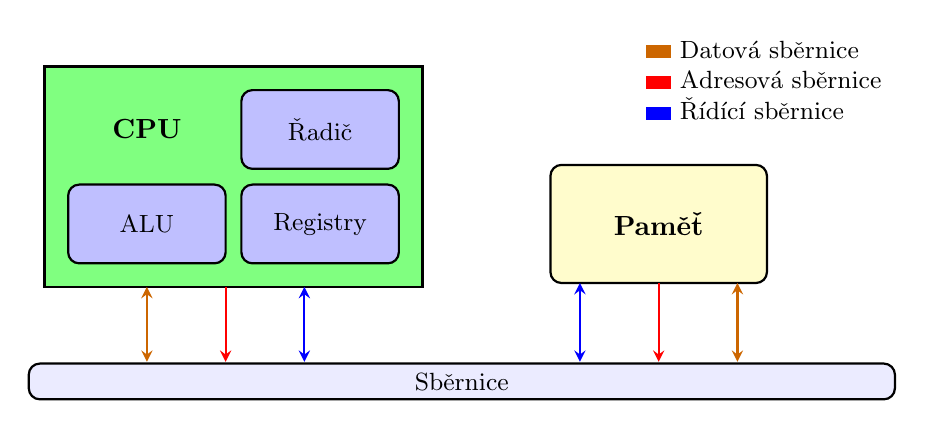
\begin{tikzpicture}[
    x=1cm, y=1cm,
    >=stealth,
    every node/.style={font=\small},
    title/.style={font=\bfseries},
    unit/.style={
        draw,
        thick,
        rounded corners,
        align=center,
        minimum width=2.25cm,
        minimum height=0.72cm
    },
    arr/.style={<->, thick}
]
    % CPU
    \draw[fill=green!50, thick] (-5.3, 4.0) rectangle (-0.5, 1.2);
    \node[font=\bfseries] at (-4, 3.2) {CPU};
    \node[unit, fill=blue!25, minimum width=2.00cm, minimum height=1.00cm] (reg) at (-1.8, 2) {Registry};
    \node[unit, fill=blue!25, minimum width=2.00cm, minimum height=1.00cm] (cont) at (-1.8, 3.2) {Řadič};
    \node[unit, fill=blue!25, minimum width=2.00cm, minimum height=1.00cm] (alu) at (-4, 2) {ALU};

    % Bus
    \node[unit, fill=blue!8, minimum width=11.00cm, minimum height=0.40cm] (bus) at (0, 0) {Sběrnice};

    % Memory
    \node[unit, fill=yellow!20, minimum width=2.75cm, minimum height=1.50cm, font=\bfseries] (mem) at (2.5,2.0) {Paměť};

    % Buses
    \draw[<->,orange!80!black, thick] (-4.0, 1.2) -- (-4.0, 0.25);
    \draw[->,red, thick] (-3.0, 1.2) -- (-3.0, 0.25);
    \draw[<->,blue, thick] (-2.0, 1.2) -- (-2.0, 0.25);

    \draw[<->,orange!80!black, thick] (3.5, 1.25) -- (3.5, 0.25);
    \draw[->,red, thick] (2.5, 1.25) -- (2.5, 0.25);
    \draw[<->,blue, thick] (1.5, 1.25) -- (1.5, 0.25);

    % Legend
    \node[anchor=north west] at (2.0, 4.5) {
        \begin{tabular}{l}
            \textcolor{orange!80!black}{\rule{1em}{0.5em}} Datová sběrnice \\
            \textcolor{red}{\rule{1em}{0.5em}} Adresová sběrnice \\
            \textcolor{blue}{\rule{1em}{0.5em}} Řídící sběrnice \\
        \end{tabular}
    };

\end{tikzpicture}
